\subsection{Competition results}
The competition took place on two dates (15th and 17th of September) and each team had to play three times against all other teams. Each simulation consisted of a of 400 steps and the team with the highest score at the end got three points for a victory. The team "MaKo" scored second with a total of 18 points. The winner 2014 was, for three times in a row now, the team from the USFC. The overall result looks like the following:
\begin{figure}[h]
	\centering
	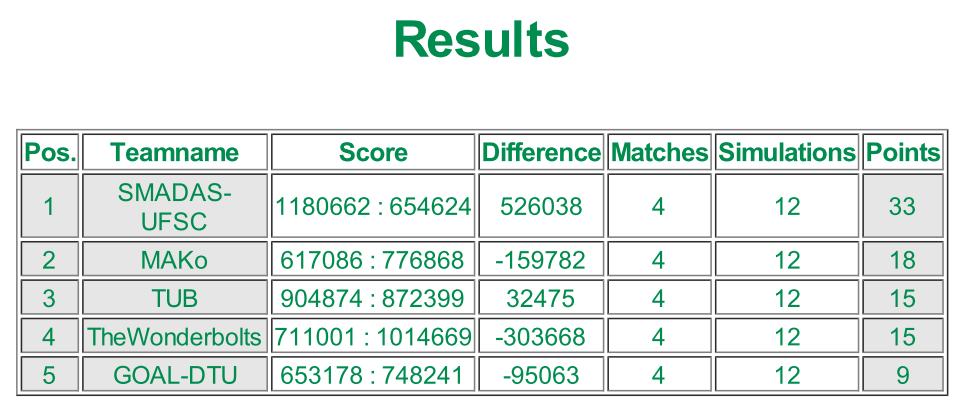
\includegraphics[width=300px]{images/con_result.png}
	\caption{MAPC 2014 result}
	\label{dis:result}
\end{figure}
Statistics of all the individual games can be found in the appendix.[reference here!!!!]

Team "MaKo" lost every second game against each opponent due to the fact that for some reason the repairer agents weren't able to repair. The reason behind this was not obvious to the team. A strategy that worked out well, was the approach to upgrade the visibility range and the strength of one saboteur agent significantly. In all matches the it was able to disable enemy agents many times and therefore disturb zones and keep the enemy repairers busy, which kept them away from building zones.

% TODO: these are from the TOC:
%What place did we rank? How did the others do? Analyse our matches shortly and point out problems we faced, how we tackled them and point out what had gone well.
